\documentclass[10pt]{scrartcl}
% \documentclass[10pt]{article}
\usepackage[T1]{fontenc}
\usepackage{amsmath,amsfonts,amssymb}
\usepackage{mathtools}
\usepackage{color,soul}
\usepackage{fullpage}
\usepackage{enumerate}
\usepackage{graphicx}
\usepackage[colorlinks=true,urlcolor=blue]{hyperref}
\usepackage{subcaption}
\usepackage{deluxetable}

\definecolor{Light}{gray}{.90}
\sethlcolor{Light}

\title{Skimmed 2D Images}
\author{Jeren Suzuki}
\date{Last Edited \today}

\begin{document}

\maketitle

\begin{figure}[!ht]
    \centering
    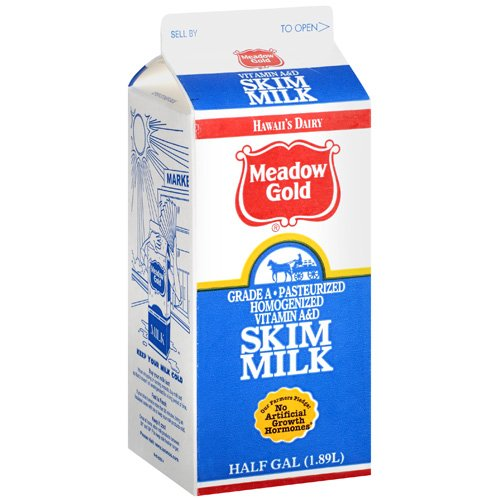
\includegraphics[width=.9\textwidth]{../plots_tables_images/skimmilk.jpg}    
\end{figure}

\clearpage

\pagenumbering{Roman}
\tableofcontents
\clearpage
\pagenumbering{arabic}

\section{Introduction} % (fold)
\label{sec:introduction}
An easier and faster way to crop our three suns in a single image is to find the brightest sun-like shape in our image, crop around it, set the area to zero, then find the next brightest sun-like shape. If we use sort to get a ``master array'' of positions and values, we can zero-out the parts of the image that are sun-like on the same array multiple times. The result is a fast and efficient cropping method. We also use the term ``skimmed'' to signify that we skim off the top 1\% of the pixels so that any extremely bright outliers will not be incorporated into our image. Actually, that's a complete lie. We only used this ``skimming'' for the old way of finding a threshold which we have proven to be replaceable by our more robust method. Keeping the carton of skim milk though.

% section introduction (end)

\section{1D Plot of a 2D image} % (fold)
\label{sec:1d_plot_of_a_2d_image}
We plot a 2D image as a 1D spectrum to identify the shapes in our 2D image.


\begin{figure}[!ht]
    \centering
    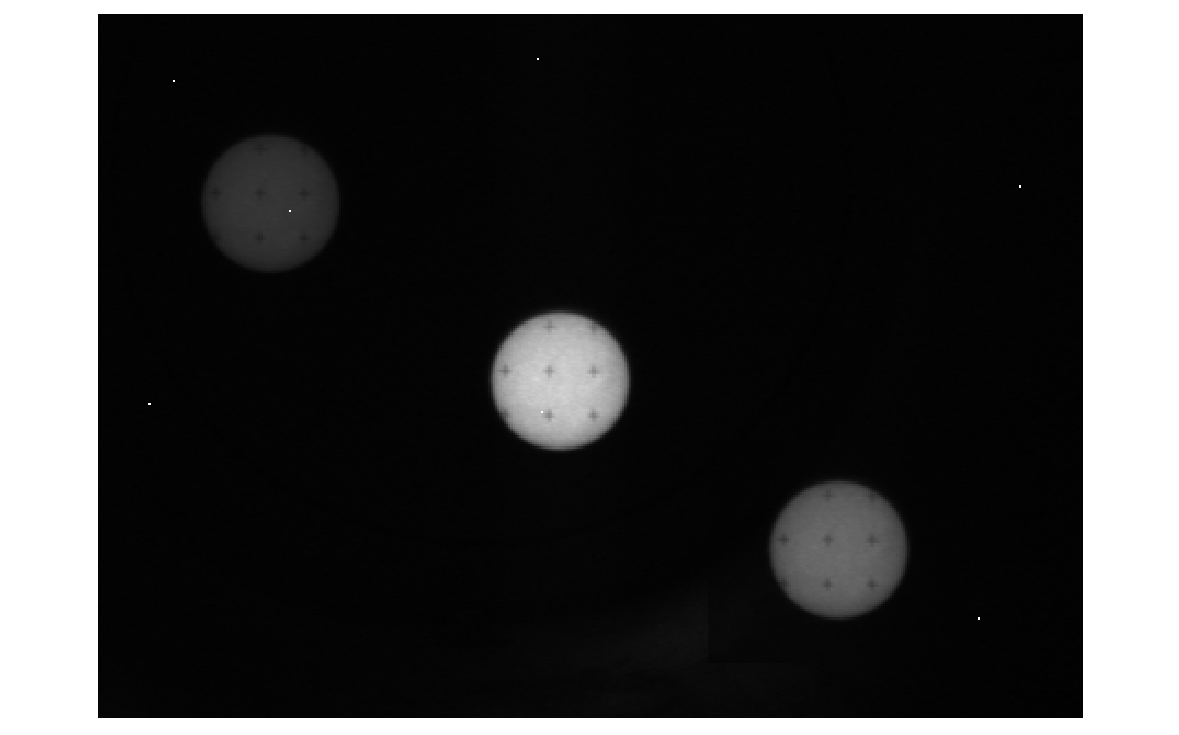
\includegraphics[width=.9\textwidth]{../plots_tables_images/raw.eps}
    \caption{The raw 2D image we started out with. There are 7 pixels in this image equal to 255, the max brightness for a byte array. These pixels simulate abnormally high values in our image as a result of bad pixels, gamma rays, etc.}
    \label{raw}
\end{figure}

Starting from Figure \ref{raw}, we plotted the lowest 99\% of the pixels when ordered by brightness to eliminate the abnormally high pixels to get Figure \ref{sorted}.

\begin{figure}[!ht]
    \centering
    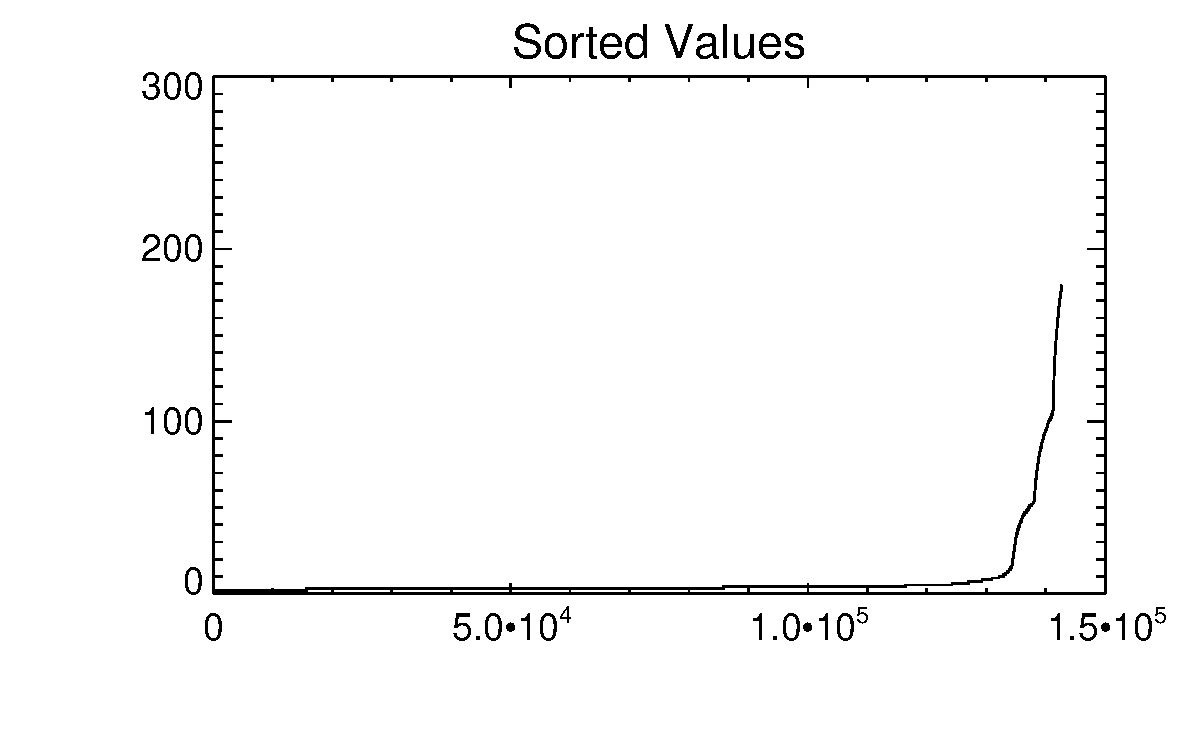
\includegraphics[width=.9\textwidth]{../plots_tables_images/sorted_array.eps}
    \caption{Lowest 99\% of sorted 2D image.}
    \label{sorted}
\end{figure}

We see three distinct humps, indicative of our three suns in the 2D image. Now, to find the boundaries where one sun ends and the other begins, we look at the derivative of Figure \ref{sorted}. However, simply taking the derivative does not result in a usable result so we must smooth our data first. I use both \texttt{\hl{smooth()}} and \texttt{\hl{ts\_smooth()}} in Figure \ref{comps}.

\begin{figure}[!ht]
    \centering 
    \hspace{-1.0in}
    \begin{subfigure}[b]{.45\linewidth}
        \centering
        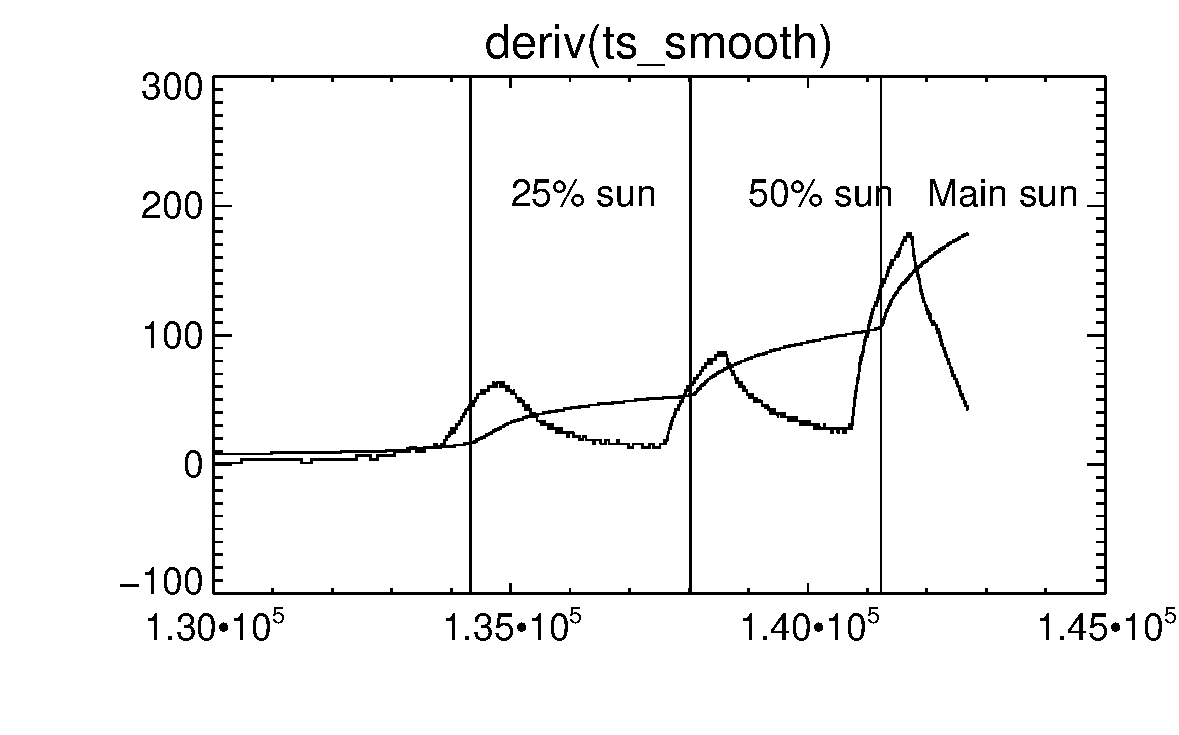
\includegraphics[width=1.3\textwidth]{../plots_tables_images/d_ts.eps}
    \end{subfigure}
    \hspace{.5in}
    \begin{subfigure}[b]{.45\linewidth}
        \centering
        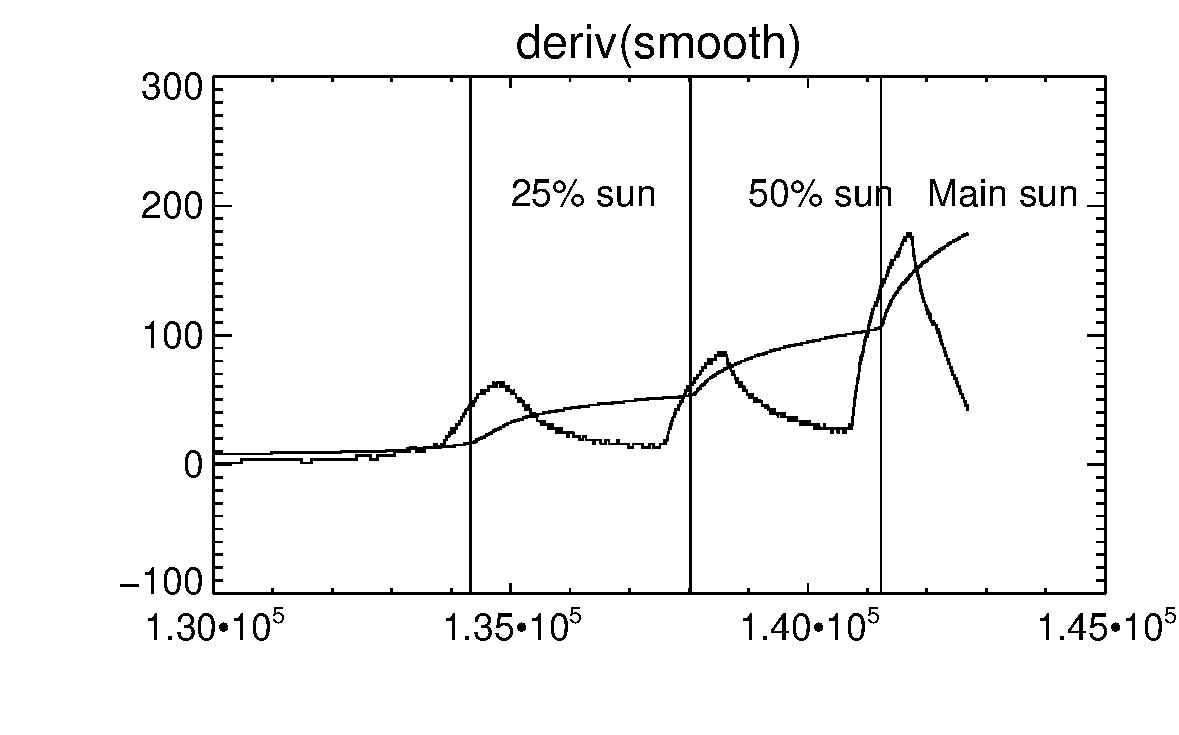
\includegraphics[width=1.3\textwidth]{../plots_tables_images/d_reg.eps}
    \end{subfigure}
   
   \hspace{-1.0in}
   \begin{subfigure}[b]{.45\linewidth}
        \centering
        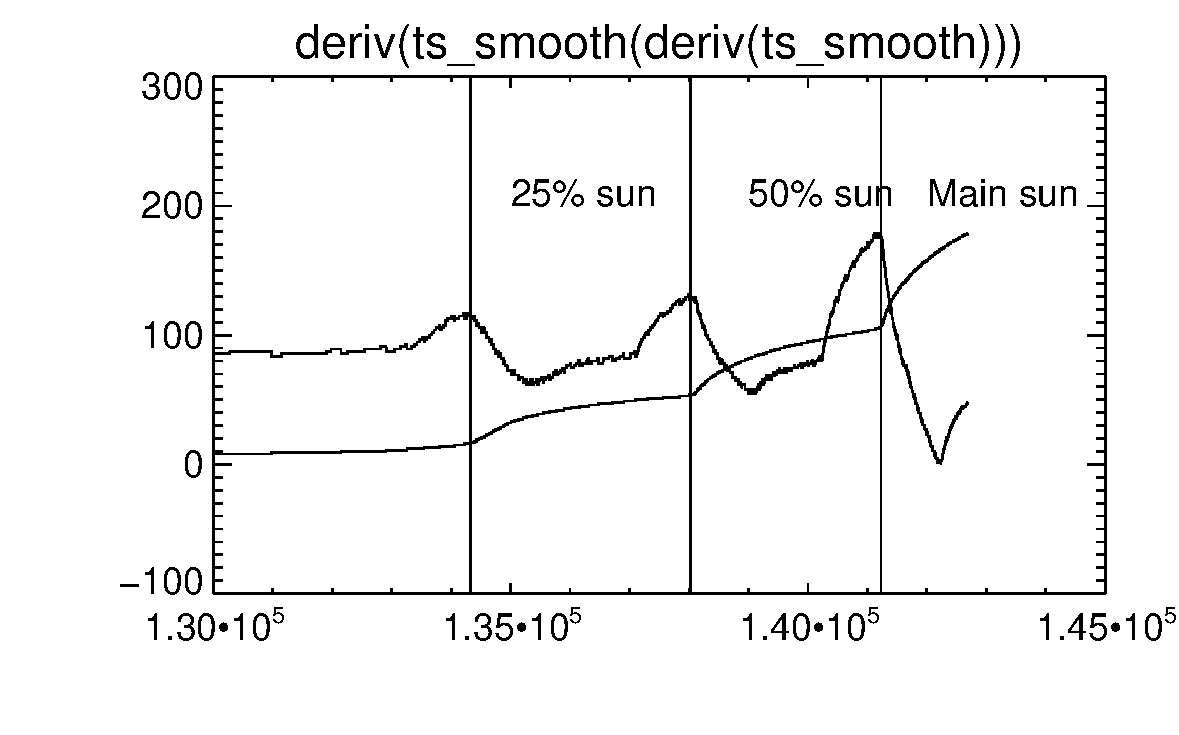
\includegraphics[width=1.3\textwidth]{../plots_tables_images/d_ts_d_ts.eps}
    \end{subfigure}
    \hspace{.5in}
    \begin{subfigure}[b]{.45\linewidth}
        \centering
        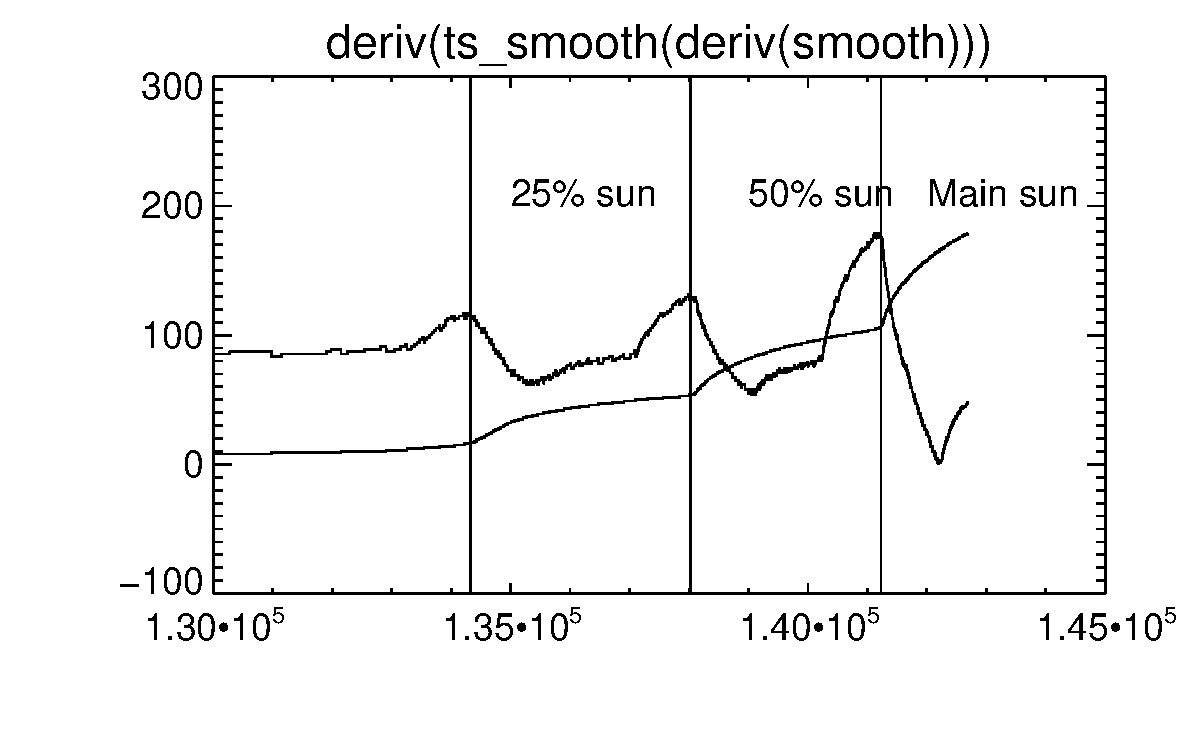
\includegraphics[width=1.3\textwidth]{../plots_tables_images/d_ts_d_reg.eps}
    \end{subfigure}

    \hspace{-1.0in}
    \begin{subfigure}[b]{.45\linewidth}
        \centering
        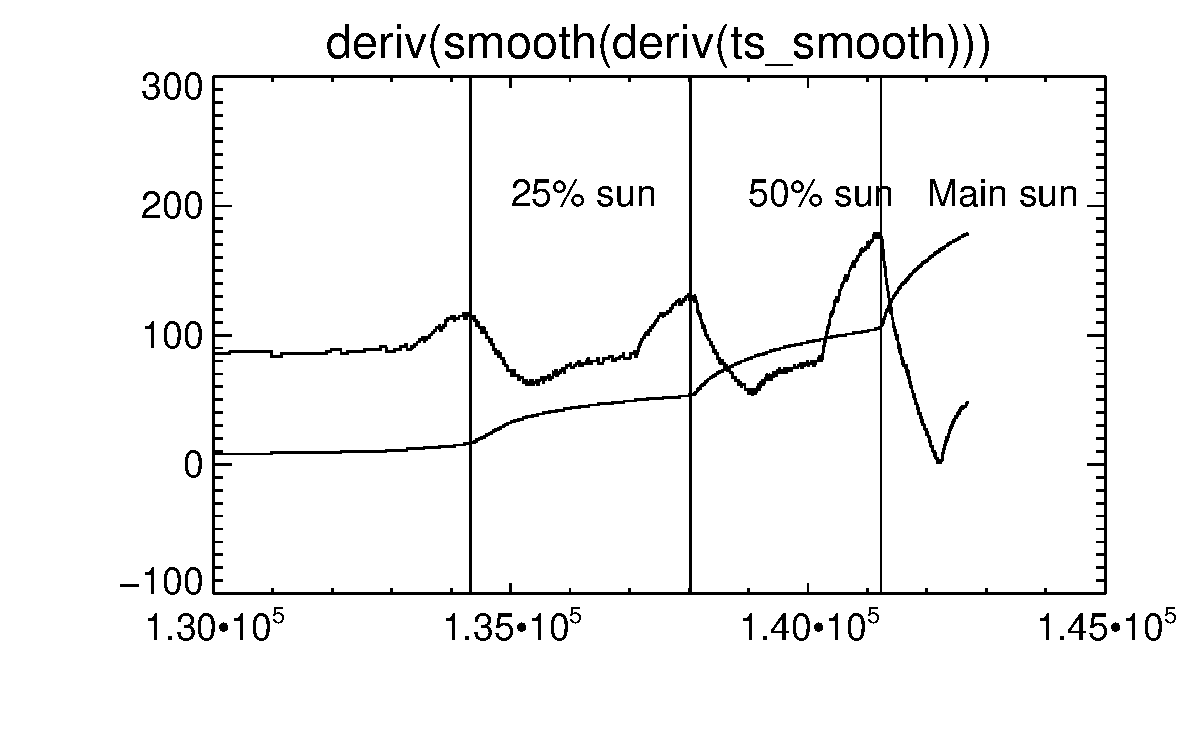
\includegraphics[width=1.3\textwidth]{../plots_tables_images/d_s_d_ts.eps}
    \end{subfigure}
    \hspace{.5in}
    \begin{subfigure}[b]{.45\linewidth}
        \centering
        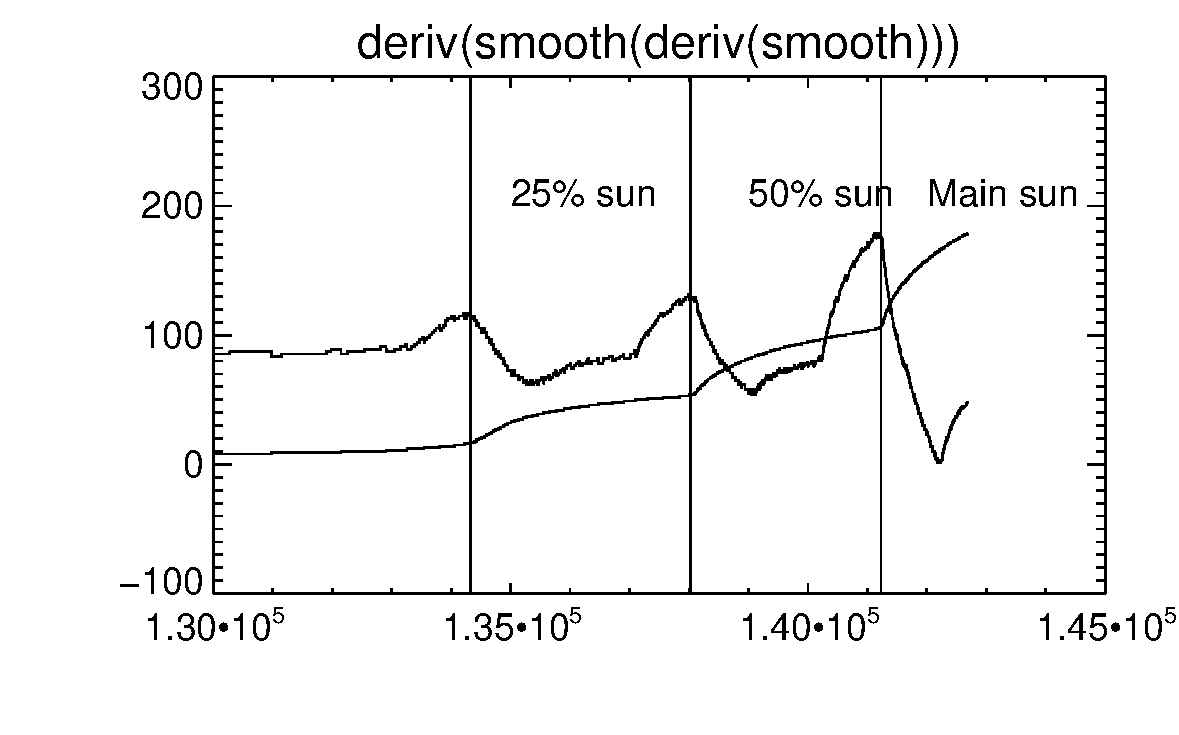
\includegraphics[width=1.3\textwidth]{../plots_tables_images/d_s_d_reg.eps}
    \end{subfigure}
    \caption{The vertical lines correspond to eyeballed boundaries of the sorted array. A large part of the left half of the array is cropped out to emphasize the shape of the humps and peaks. The derivative has been scaled to within the max/min of the starting master array. The width of the smoothing filter is 1000 wide.}
    \label{comps}
\end{figure}

It turns out that \texttt{\hl{ts\_smooth}} takes an incredibly long time to run when the order of the autoregressive model is greater than 10. As such, I chose an order of 3 so that it didn't take too long. Even then, running a simple \hl{\texttt{smooth()}} filter results in some pretty good plots. It's important to note that the derivative must be smoothed before I can take another another derivative; also, it doesn't seem to matter if I use \texttt{\hl{ts\_smooth}} or \hl{\texttt{smooth()}} when taking the second smooth.

% section 1d_plot_of_a_2d_image (end)


\section{Drawbacks} % (fold)
\label{sec:drawbacks}
    
    The biggest problem with this method is that the pixel values overlap somewhat with different regions. Say the brightest region, region 1, is in the center of our image. Region 2 is at a brightness 50\% of the main sun. Say we now arrange the 2D plot as a 1D array and see two bumps, one for each solar region. Now, region 2 is intrinsically dimmer than region 1, which means there are going to be pixels in region 2 that will be comparative to the dark limb pixels of region 1. Since our 1D array (now that it's sorted, especially) has no spatial information, we cannot tell two pixels apart that have the same value but are in different regions. 

    Another obvious drawback is the necessity of a \hl{\texttt{smooth}} filter. Not only does this require parameterization, it blurs out our data set. Instead of applying a filter, we can attempt to use a histogram plot to isolate the shape of our sorted main array. Figure \ref{histozoom} shows the structure of our three suns.

\begin{figure}[!ht]
    \centering
    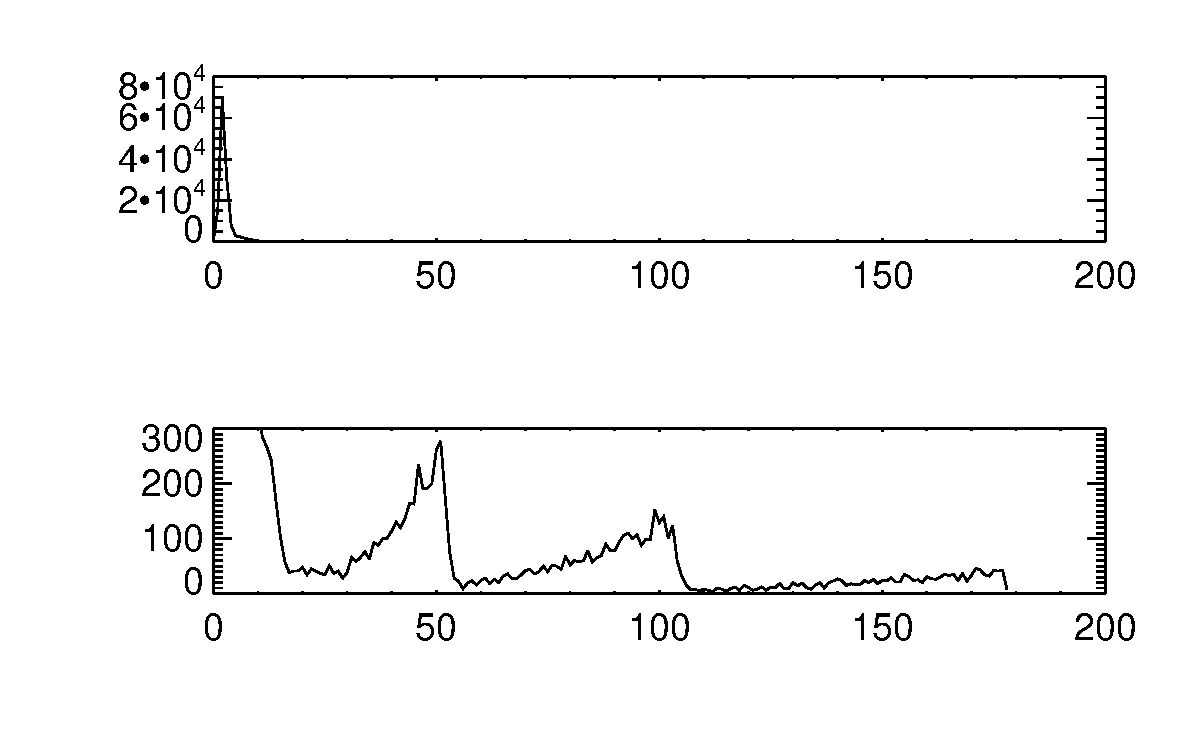
\includegraphics[width=.9\textwidth]{../plots_tables_images/histozoom.eps}
    \caption{The top is the histogram of the sorted array. The bottom is the same plot but zoomed to a y-range of [0:300].}
    \label{histozoom}
\end{figure}

    Bring your attention to the double peak shape around the 50 tick on the x-axis. This is probably the result of the aforementioned inability to extract spatial data from a sorted array. The low-pixel values from one region are being binned into the same bin as the low-pixel values from another region. 

% section drawbacks (end)

\section{This Plot Says it All} % (fold)
\label{sec:this_plot_says_it_all}

    I wanted to see how many pixels were being counted in the wrong region, henceforth called ``leakage-pixels''. It turns out that it's not easy to see but it \emph{is} obvious that there are a fair number of them. Depending on how we handle our cropping however, we may not have to worry about it. For example, after we find the center of the brightest region, we set the cropped region to zero so that the middle row thing in the top two plots of Figure \ref{saysitall} is blanked out horizontally. If that's the case, then when we look vertically in the second brightest region, we shouldn't have to worry about counting any pixels from the first region (since it's cropped out). 

\begin{figure}[!ht]
    \centering
    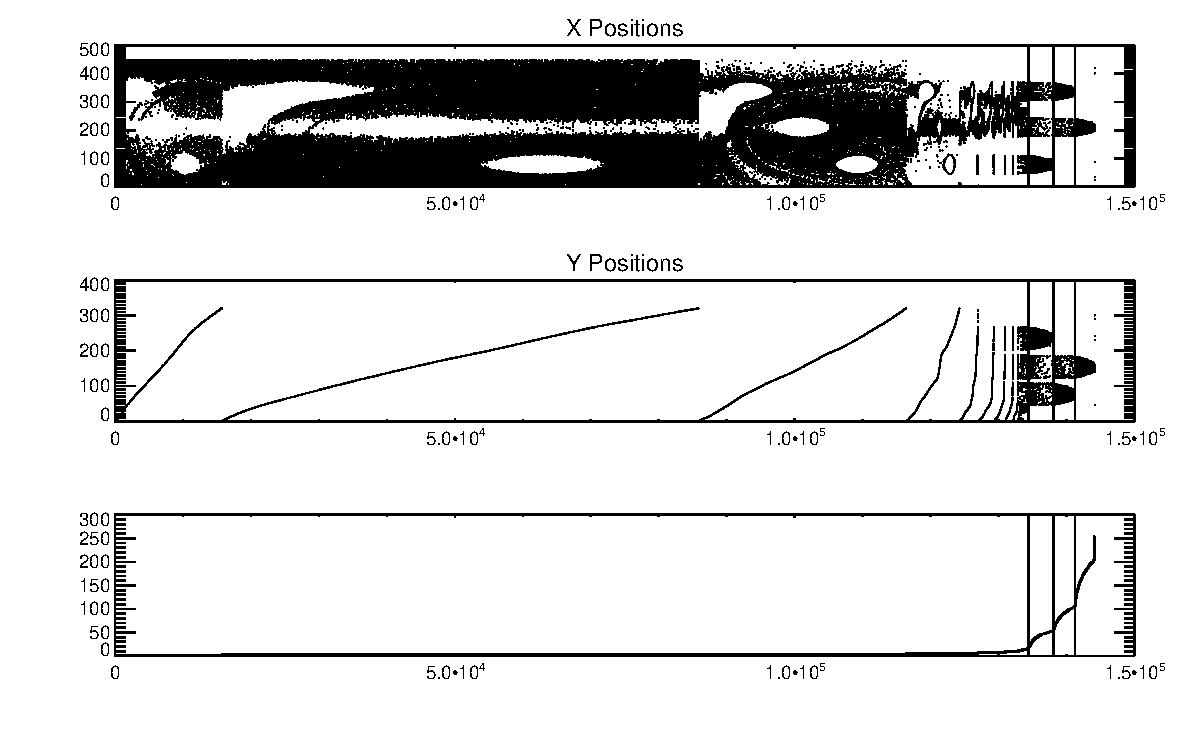
\includegraphics[width=.9\textwidth]{../plots_tables_images/saysitall.eps}
    \caption{This plot reveals that when sorted, the regions bounded by the vertical lines (which are artificially places, not the result of any computation) include pixels from neighboring regions. For high-value pixels, i.e., the region bounded by the rightmost vertical line and the last element of the sorted array, the x and y positions are completely (no vertical dots) isolated from other regions. When we look at the middle region, we see that low-value pixels from the brightest region(most likely dark limb pixels) are being sorted into the middle region of the sorted array. The worst case scenario is the left-most region which has pixels from both the first and second regions. This approach, however, is without the inclusion of cropping and then setting the cropped area to zero.}
    \label{saysitall}
\end{figure}

I also wanted to see what it would look like when the suns are lined up in a single axis: see Figure \ref{inaline}

\begin{figure}[!ht]
    \centering
    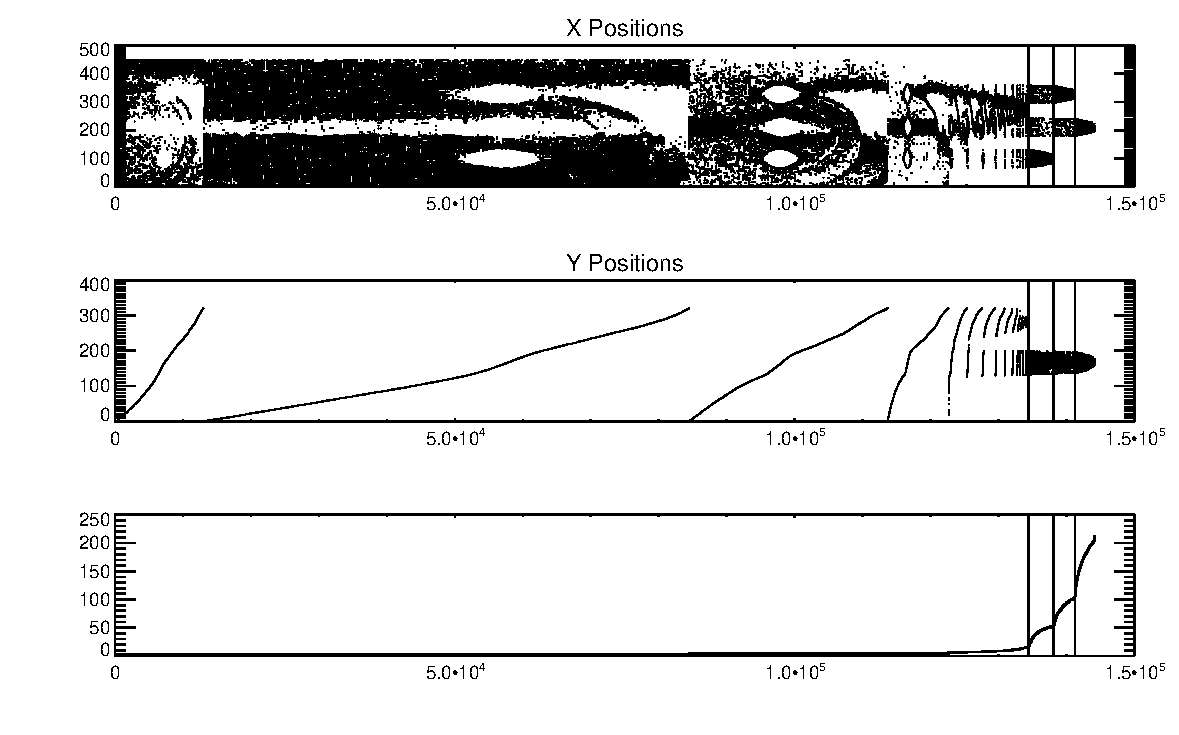
\includegraphics[width=.9\textwidth]{../plots_tables_images/inaline.eps}
    \caption{The suns are lined up vertically}
    \label{inaline}
\end{figure}

% section this_plot_says_it_all (end)

\section{Some Numbers} % (fold)
\label{sec:some_numbers}
Using the above methods, we find peaks of the second derivative of the smoothed 2D$\rightarrow$1D array. Using the peak positions, we return the value of the sorted array at that peak position and set that to be a threshold. The result is a set of three thresholds based on the shape of the 1D image. We keep our code identical and only change the threshold value. Table \ref{threshcomp} shows that the thresholds we find are good! There is one small note however, the exactly position of the peak is not used, but rather the position +.1\% of the total number of pixels in the 1D array. The problem was that if we did simply return the sorted array value as a threshold, we'd get cropping errors. Adding a little bit to the threshold value is safe, however, since it reduces the number of pixels in our centering mask. The less pixels there are, the higher on the dome-shape we lie, which means the more circular our mask is. A more circular mask means a more accurate center position to use for our limb-fitting program. 

\begin{deluxetable}{rllr}
\tablecaption{Center Positions Using Different Thresholds}
\tablewidth{0pt}
\tablehead{
    \colhead{Sun Brightness (\%)} %
&   \colhead{X Position} %
&   \colhead{Y Position} %
&   \colhead{Threshold} %
}
\startdata
& & & Old\\
\hline
100
& 210.50238
& 154.27054
& 116.35\\
%
50
& 337.80600
& 76.894958
& 76.5\\
%
25
& 78.683426
& 235.11536
& 35.8\\
\hline
& & & New\\
\hline
100
& 210.48686
& 154.25601
& 123\\
%
50
& 337.91956
& 77.234901
& 62\\
%
25
& 78.887283
& 234.69048
& 20
\enddata
\label{threshcomp}
\end{deluxetable}

% section some_numbers (end)

\section{Taking this Method Further} % (fold)
\label{sec:taking_this_method_further}

    Once we have the sorted array we can try to do cool things with it. For example, we can attempt to find the quick centers of the three suns. We can do this by partitioning the sorted array into three parts, 1 for each sun. We average the positions of all pixels above a certain threshold and then zero-out a box that is 120x120 pixels wide centered at the recently-found center. We repeat the same process, computing the average position of all pixels above a certain threshold. We don't have to worry about the darker limb pixels of the main sun because we have set all the pixels around the center to 0. Figure \ref{goodenough} illustrates how accurate the process is to find centers. 

\begin{figure}[!ht]
    \centering
    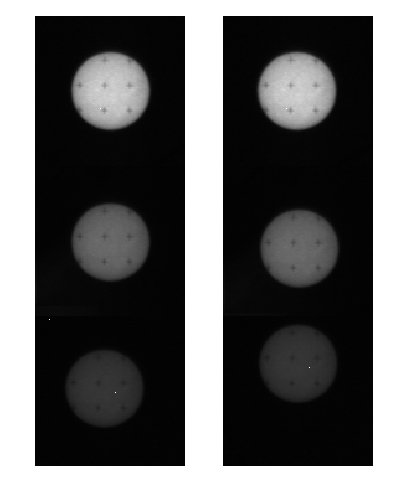
\includegraphics[width=.9\textwidth]{../plots_tables_images/goodenough.eps}
    \caption{The left column are the cropped regions found by our previous method (scanning in a circle after we found the main sun position). The right column are the cropped regions found by the method of averaging positions of our sorted array.}
    \label{goodneough}
\end{figure}

\begin{figure}[!ht]
    \centering
    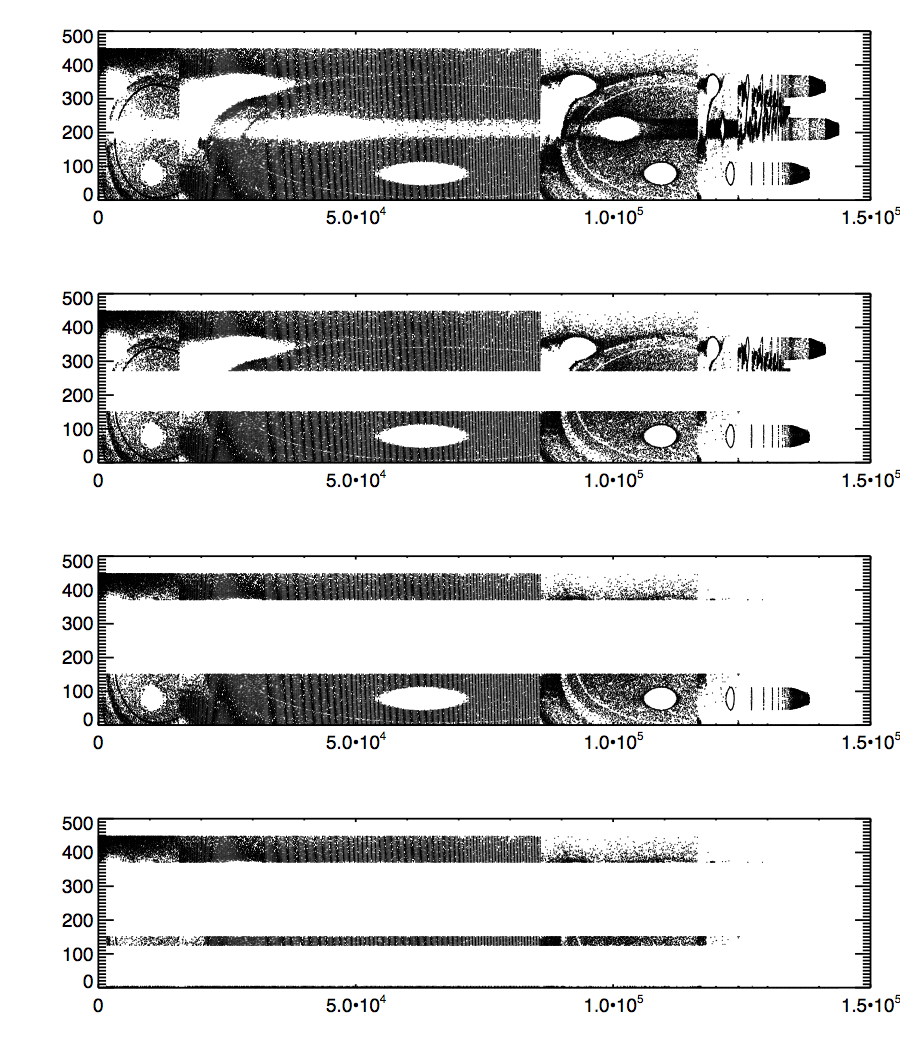
\includegraphics[width=.9\textwidth]{../plots_tables_images/quickcenters.eps}
    \caption{The top row are the x positions plotted against the sorted pixel values. In the second row we find the center of the brightest region and set the x (and y) positions in a 60-wide window to 0. In the third region we find the pixel positions of the second brightest region and repeat the process of zeroing out neighboring pixels. In the third row, only the dimmest region remains, free from the dim pixels of the first two regions.}
    \label{quickcenters}
\end{figure}

\begin{deluxetable}{lcll}
\tablecaption{Center Positions Using Different Methods}
\tablewidth{0pt}
\tablehead{
    \colhead{Type} %
&   \colhead{Sun Brightness (\%)} %
&   \colhead{X Position} %
&   \colhead{Y Position} %
}
\startdata
\hline
Old
& 100
& 210.174
& 153.800\\
%
"
& 50
& 337.717
& 76.7694\\
%
"
& 25
& 83.4095
& 232.106\\
\hline
New
& 100
& 211.2756
& 153.1704\\
%
"
& 50
& 336.4977
& 82.6384\\
%
"
& 25
& 78.4613
& 212.2920
\enddata
\label{numethod}
\end{deluxetable}


% section taking_this_method_further (end)

\end{document}










